\documentclass[12pt,svgnames,table]{beamer}
\usetheme{progressbar}

\usepackage[utf8x,utf8]{inputenc}
\usepackage{tikz}
\usetikzlibrary{decorations.pathmorphing}
\usepackage{xcolor}
\usepackage{amsmath,amsfonts,amsthm, amssymb}
\usepackage[babel=true]{csquotes}
\usepackage{etoolbox}
\usepackage{dsfont}
\usepackage{chngpage}


\usepackage{graphics} %% TOUT NEW!!
\usepackage{pgfplots} %% TOUT NEW!!  virer si pbm

\usetikzlibrary{shapes,snakes}

%\usepackage{txfonts}
%\usepackage{MnSymbol} % symbol independent
\newcommand{\paren}[1]{\left( \left. #1 \right. \right)} 
\newcommand{\croch}[1]{\left[ \left. #1 \right. \right]} 
\newcommand{\set}[1]{\left\{ \left. #1 \right. \right\}}
\newcommand{\sachant}{\, \right| \left. \,}
\newcommand{\nico}[1]{ }
\newcommand{\nicoo}[1]{#1}
% Modifiez ou necessaire:
% titre de these/topo

\title{
\vspace{0.7cm}\\
PIR : Mixed-Initiative Mission}

\normalsize
\author{\vspace{2cm} \textbf{Thomas Vagneron}}
% X=annee de these, Y=departement
\def\aboutauthor{\vspace{0.2cm}\hspace{-2.55cm} 
%under \textbf{D.Dubois}, \textbf{J-L.Farges} and \textbf{F.Teichteil-K\"onigsbuch} supervision\\
%\vspace{0.1cm}\hspace{-2.4cm} \textbf{doctoral school:} EDSYS \hspace{0.2cm} \textbf{institution:} ISAE--SUPAERO\\
%\vspace{0.1cm}\hspace{-3.2cm}\textbf{laboratory:} ONERA--The French Aerospace Lab\\ 
%\vspace{0.5cm} \hspace{0.2cm} 
\includegraphics[scale=0.45]{logo2015} \hspace{4.8cm}
%\begin{tikzpicture}
%\node[opacity=1] at (0,0) {\includegraphics[scale=0.35]{Logo_EDSYS2}};
%\end{tikzpicture}
}

% directeur de these
%\def\directeur{Toulouse}
% encadrant; s'il n'y a pas d'encadrant, veuillez commenter la ligne ci-dessous
%\def\encadrant{DCSD}


% Debut du documment
\begin{document}

% la premiere page
{
\usebackgroundtemplate{
\includegraphics[width=\paperwidth,height=\paperheight]{image_fond}} 
\begin{frame}[plain]
	\titlepage
\end{frame}
}
\section[summary]{summary}
\begin{frame}
\frametitle{Summary}

\end{frame}
\section[context]{Context and Goal}

\begin{frame}
\frametitle{\insertsection} 
\framesubtitle{\footnotesize Human-machine systems}
\begin{block}{Increasing use of automated systems}
aircrafts, cars, unmanned vehicles (military operation, contaminated area), ... \\
\end{block}
\visible<2->{
\begin{itemize}
\item \textbf{Increasingly autonomous robots:}\\ 
technical advances in AI, machine learning, vision, decision ...
%deterministic behavior conditional to feedbacks/observations (policies)
\visible<3->{
\item \textbf{Human operator still vital:}\\
%more powerful for a vast majority of tasks 
- produces tactical and ethical decisions \\
- handles complex/unknown situations/systems
%(robot can apply optimal decisions for known systems)
}
\end{itemize}
}
\visible<4->{
\begin{alertblock}{}
Human factors involved in $80\%$ of AAVs accidents! \cite{Williams04asummary}
\end{alertblock}
}
\end{frame}

\begin{frame}
\frametitle{\insertsection} 
\framesubtitle{\footnotesize Human operator weaknesses}
\textbf{Potential effects of a mission on human operators:}
\begin{itemize}
\item stress (danger, pressure)
\item workload (multi-task, hard tasks)
\item fatigue, boredom (long mission)
\end{itemize}
\visible<2->{
\textbf{Consequences:}
\begin{itemize}
\item mental confusion
\item attentional tunneling
\item mind wandering
\item lower vigilance
\item ...
\end{itemize}
}
\visible<2->{
\begin{alertblock}{}
\center increase in accident risk resulting in mission fails 
\end{alertblock}
}
\end{frame}
\begin{frame}
\frametitle{\insertsection}
\framesubtitle{\footnotesize use of human state feedbacks!}
\begin{block}{Human operators equipped with sensors}
\center data from the human operator state can\\  
\textbf{refine supervision of human-robot team}
\end{block}
\visible<2->{
\begin{itemize}
\item \cite{Souza:2015:MTS:2921564.2921916} target identification task (ground robot)\\ 
- \textbf{devices:} eye tracking + electrocardiography\\% (ECG)\\
- \textbf{human state:} \textit{cognitive availability} {\color{DodgerBlue!70} estimation}\\ 
- \textbf{superv. validation:} {\color{DodgerBlue!70} simulations} of the system\\
\hspace{3.8cm} (including human behavior)
\end{itemize}
}
\visible<3->{
\begin{itemize}
\item \cite{DBLP:2016:conf/iros/GateauCLD16} search and rescue task (AAVs)\\ 
- \textbf{device:} eye tracking\\
- \textbf{human state:} \textit{current human task} {\color{DodgerBlue!70} = } human gaze \\% (deterministic)\\
- \textbf{superv. validation:} tested on 10 {\color{DodgerBlue!70} volunteers } 
\end{itemize}
}
\end{frame}
%%%%%%%%%%%%%%%%%%%%%%%%%%%%%%%%%%%%%%%%%%%%%%%%%%%%%%%%%%%%%%%%%%%%%%
\begin{frame}
\frametitle{\insertsection}
\framesbtitle{\footnotesize The Project}
\begin{figure}
  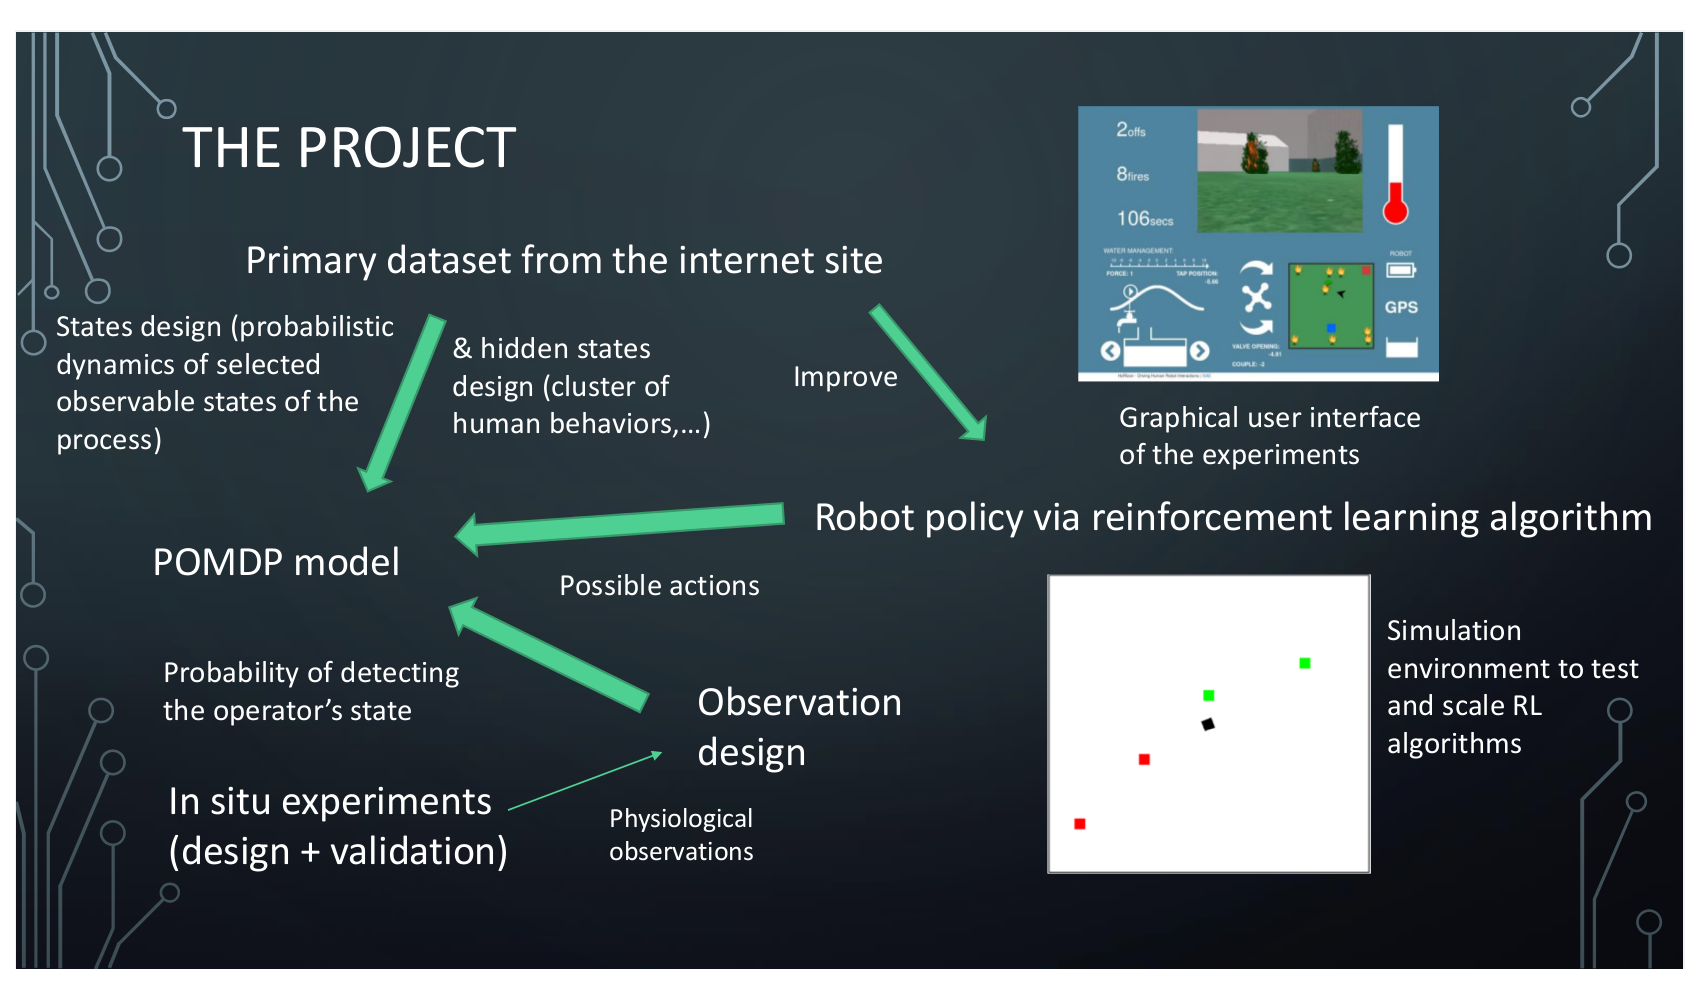
\includegraphics[scale = 0.3]{Schema.png}
  \label{fig:my-figure}
\end{figure}
\end{frame}

\begin{frame}
\frametitle{\insertsection}
\framesbtitle{\footnotesize User Interface}
\begin{figure}
  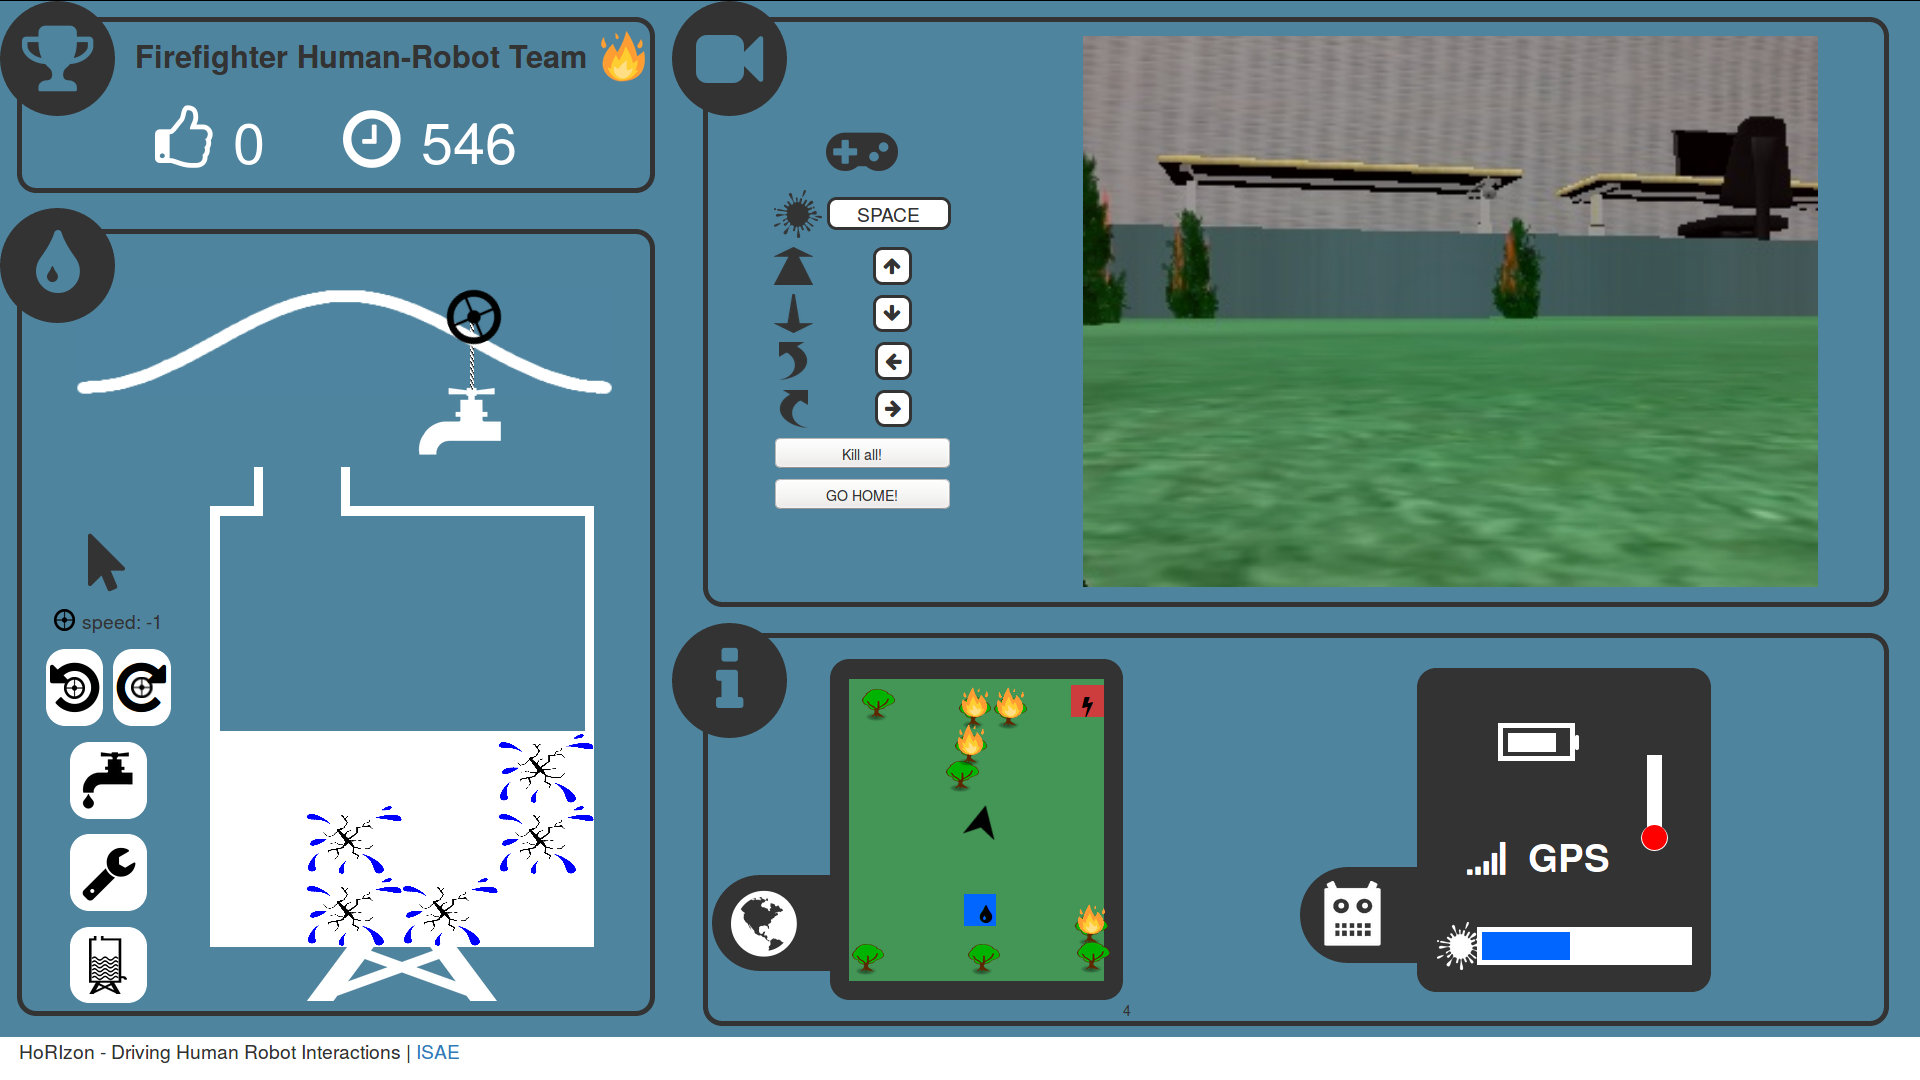
\includegraphics[scale = 0.3]{Website.png}
  \label{fig:my-figure}
\end{figure}
\end{frame}

\section[thory]{Theory}

\begin{frame}
\frametitle{\insertsection}
\framesbtitle{\footnotesize History}
\textbf{Domain's birth} : late 70's by the encounter of
\begin{itemize}
\item computational neuroscience 
\item experimental psychology
\item dynamic programming
\end{itemize}
\visible<2->{
\begin{block}{An approach to experimental psychology : Law of effects (Thorndike, 1911)}
"Of several responses made to the same situation, those which are accompanied or closely followed by satisfaction to the animal will, other things being equal, be more firmly connected with the situation, so that, when it recurs, they will be more likely to recur : those which accompanied or closely followed by discomfort to the animal will, other things being equal, have their connections with that situation weakened, so that, when it recurs, they will be less likely to occur. The greater the satisfaction or discomfort, the greater the strengthening or weakening of the bond".
\end{block}
}
\end{frame}

\begin{frame}
\frametitle{\insertsection}
\framesbtitle{\footnotesize Reinforcement Learning}
\begin{block}{What is Reinforcement Learning?}
It is an approach, here computational, to decision-making, understanding and goal-directed learning. 
\end{block}
\visible<2->{
\textbf{What does it needs?}
The definition of the interactions between a learning agent and its environment.
\begin{itemize}
 \item the states
 \item the actions
 \item the rewards
\end{itemize}
}

%%%%%%%%%%%%%%%%%%%%%%%%%%%%%%%%%%%%%%%%%%%%%%%%%%%%%%%%%%%%%%%%%%%%%%%



\begin{frame}
        \frametitle{\hspace{0.3cm} 
\includegraphics[scale=0.35,trim= 0 0 0 -0.3cm]{logo2015} }
	\vspace{-0.2cm}
	\bibliographystyle{alpha}	
	{\tiny        
		\bibliography{main}
	}
	\vspace{0.2cm}
	\hspace{5cm} {\huge \textbf{Thank you!} }
\end{frame}


%}
\end{document}
